%%%%%%%%%%%%%%%%%%%%%%%%%%%%%%%%%%%%%%%%%%%%%%%%%%%%%%%%%%%%
%%  This Beamer template was created by Cameron Bracken.
%%  Anyone can freely use or modify it for any purpose
%%  without attribution.
%%
%%  Last Modified: January 9, 2009
%%

\documentclass[xcolor=x11names,compress]{beamer}

%% General document %%%%%%%%%%%%%%%%%%%%%%%%%%%%%%%%%%
\usepackage{graphicx}
\usepackage{tikz}
\usepackage[canadian]{babel}
\usepackage[utf8]{inputenc}
\usepackage{amsmath,amssymb}
\usepackage{mathtools}
\usepackage[ruled,vlined,linesnumbered]{algorithm2e}
\usepackage{epstopdf}
\usepackage{hyperref}
\usepackage[export]{adjustbox}
\usepackage{animate}
\usepackage{minted}
\usepackage{xcolor}
\usepackage{pgfplots}
\usetikzlibrary{calc}
\graphicspath{{img/}}
%%%%%%%%%%%%%%%%%%%%%%%%%%%%%%%%%%%%%%%%%%%%%%%%%%%%%%

\DeclareMathOperator*{\argmax}{arg\,max}
\DeclareMathOperator*{\argmin}{arg\,min}
%% Beamer Layout %%%%%%%%%%%%%%%%%%%%%%%%%%%%%%%%%%
\useoutertheme[subsection=false,shadow]{miniframes}
\useinnertheme{default}
\usefonttheme{serif}
\usepackage{palatino}
\urlstyle{same}
\setbeamerfont{title like}{shape=\scshape}
\setbeamerfont{frametitle}{shape=\scshape}

\setbeamercolor*{lower separation line head}{bg=DeepSkyBlue4} 
\setbeamercolor*{normal text}{fg=black,bg=white} 
\setbeamercolor*{alerted text}{fg=red} 
\setbeamercolor*{example text}{fg=black} 
\setbeamercolor*{structure}{fg=black} 
 
\setbeamercolor*{palette tertiary}{fg=black,bg=black!10} 
\setbeamercolor*{palette quaternary}{fg=black,bg=black!10} 

\renewcommand{\(}{\begin{columns}}
\renewcommand{\)}{\end{columns}}
\newcommand{\<}[1]{\begin{column}{#1}}
\renewcommand{\>}{\end{column}}
\setbeamertemplate{navigation symbols}{}

\setbeamerfont{footline}{size=\fontsize{6}{0}\selectfont}
\setbeamercolor{footline}{fg=black!50}

\setbeamertemplate{footline}{
	\parbox{\paperwidth}{\hspace*{5pt}\url{http://www.cs.toronto.edu/~frossard}\hfill
		\insertframenumber/\inserttotalframenumber\hspace*{5pt}}
	}
\usemintedstyle{tango}
%%%%%%%%%%%%%%%%%%%%%%%%%%%%%%%%%%%%%%%%%%%%%%%%%%

\begin{document}
%%%%%%%%%%%%%%%%%%%%%%%%%%%%%%%%%%%%%%%%%%%%%%%%%%%%%%
%%%%%%%%%%%%%%%%%%%%%%%%%%%%%%%%%%%%%%%%%%%%%%%%%%%%%%
\section{\scshape Introduction}
\begin{frame}
	\title{Introduction to Machine Learning}
	\subtitle{Convolutional Neural Networks}
	\author{
		Davi Frossard\\
		{\it Federal University of Espirito Santo \\ University of Toronto}\\
	}
	\date{
		\vspace{-2em}\\
		\includegraphics[width=0.6\columnwidth]{neuralstyle.jpg}\\[-1ex]
		{\tiny Credit: {\itshape \url{https://github.com/awentzonline/image-analogies}}}
		\\
		\today
	}
	\titlepage
\end{frame}

%%%%%%%%%%%%%%%%%%%%%%%%%%%%%%%%%%%%%%%%%%%%%%%%%%%%%%
%%%%%%%%%%%%%%%%%%%%%%%%%%%%%%%%%%%%%%%%%%%%%%%%%%%%%%
\begin{frame}{Summary}
	\tableofcontents
\end{frame}

%%%%%%%%%%%%%%%%%%%%%%%%%%%%%%%%%%%%%%%%%%%%%%%%%%%%%%
%%%%%%%%%%%%%%%%%%%%%%%%%%%%%%%%%%%%%%%%%%%%%%%%%%%%%%
\section{\scshape Filters}
\begin{frame}{Filters}
	\begin{itemize}
		\item We can extract features from an image by convolving a filter with it.
		\item There are many manually engineered filters that extract certain features from images (edges, blobs, etc).
		\item Others manipulate the image (blur, sharpen, identity, etc).
		\item In general, hand crafting feature extractors is tiresome.
	\end{itemize}
\end{frame}

%%%%%%%%%%%%%%%%%%%%%%%%%%%%%%%%%%%%%%%%%%%%%%%%%%%%%%
%%%%%%%%%%%%%%%%%%%%%%%%%%%%%%%%%%%%%%%%%%%%%%%%%%%%%%
\subsection{Sobel Filter}
\begin{frame}{Filters}
	\begin{itemize}
		\item Horizontal Sobel Filter
	\end{itemize}
	\begin{center}
		\only<-1>{
			\begin{tabular}{rl}
				\raisebox{-.5\height}{\includegraphics[width=0.7\columnwidth]{reitoria}}
				&
				$\star \begin{bmatrix}1 & 2 & 1 \\ 0 & 0 & 0\\ -1&-2&-1\end{bmatrix}$
			\end{tabular}}
		\only<2->{
			\includegraphics[width=0.8\columnwidth]{reitoria_x}
		}
	\end{center}
\end{frame}

%%%%%%%%%%%%%%%%%%%%%%%%%%%%%%%%%%%%%%%%%%%%%%%%%%%%%%
%%%%%%%%%%%%%%%%%%%%%%%%%%%%%%%%%%%%%%%%%%%%%%%%%%%%%%
\begin{frame}{Filters}
	\begin{itemize}
		\item Vertical Sobel Filter
	\end{itemize}
	\begin{center}
		\only<-1>{
			\begin{tabular}{rl}
				\raisebox{-.5\height}{\includegraphics[width=0.7\columnwidth]{reitoria}}
				&
				$\star \begin{bmatrix}1 & 0 & -1 \\ 2 & 0 & -2\\ 1&0&-1\end{bmatrix}$
			\end{tabular}}
		\only<2->{
			\includegraphics[width=0.8\columnwidth]{reitoria_y}
		}
	\end{center}
\end{frame}

%%%%%%%%%%%%%%%%%%%%%%%%%%%%%%%%%%%%%%%%%%%%%%%%%%%%%%
%%%%%%%%%%%%%%%%%%%%%%%%%%%%%%%%%%%%%%%%%%%%%%%%%%%%%%
\section{\scshape Convolution}
\subsection{Examples}
\begin{frame}{Convolution}
	\begin{itemize}
		\item Convolution Operation on Images
	\end{itemize}
	\begin{center}
		\resizebox{!}{0.65\columnwidth}{
			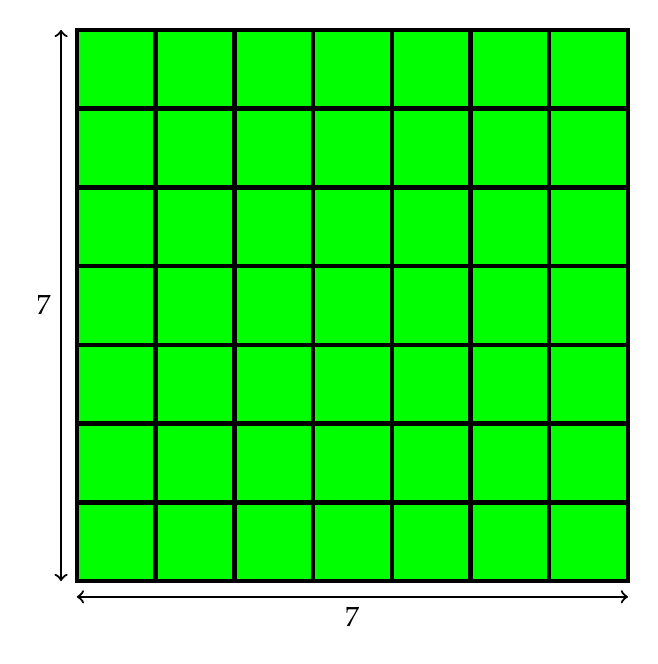
\begin{tikzpicture}
				\foreach \idy [count=\j] in {4,...,0}
				{
					\foreach \idx [count=\i] in {0,...,4}
					{
						\pgfmathparse{int(\j*5-5+\i)}
						\only<\pgfmathresult>{
							\draw[fill=green, draw=black, ultra thick] (\idx,\idy) rectangle (\idx+3,\idy+3);
						}
						\typeout{\pgfmathresult}
					}
				}
				\foreach \y in {1,...,7} {
					\foreach \x in {1,...,7} {
						\draw [draw=black, ultra thick] (\x-1,\y-1) rectangle (\x,\y);
					}
				}
				\draw[yshift=-0.2cm, thick, <->] (0,0) -- (7,0) node[midway,below] {7};
				\draw[xshift=-0.2cm, thick, <->] (0,0) -- (0,7) node[midway,left] {7};
			\end{tikzpicture}
		}
	\end{center}
\end{frame}

%%%%%%%%%%%%%%%%%%%%%%%%%%%%%%%%%%%%%%%%%%%%%%%%%%%%%%
%%%%%%%%%%%%%%%%%%%%%%%%%%%%%%%%%%%%%%%%%%%%%%%%%%%%%%
\begin{frame}{Convolution}
	\begin{itemize}
		\item 7x7 input.
		\item 3x3 filter.
		\item Stride of 1.
		\item \textbf{5x5 output}.
	\end{itemize}
\end{frame}

%%%%%%%%%%%%%%%%%%%%%%%%%%%%%%%%%%%%%%%%%%%%%%%%%%%%%%
%%%%%%%%%%%%%%%%%%%%%%%%%%%%%%%%%%%%%%%%%%%%%%%%%%%%%%
\begin{frame}{Convolution}
	\begin{itemize}
		\item Convolution Operation on Images
	\end{itemize}
	\begin{center}
		\resizebox{!}{0.65\columnwidth}{
			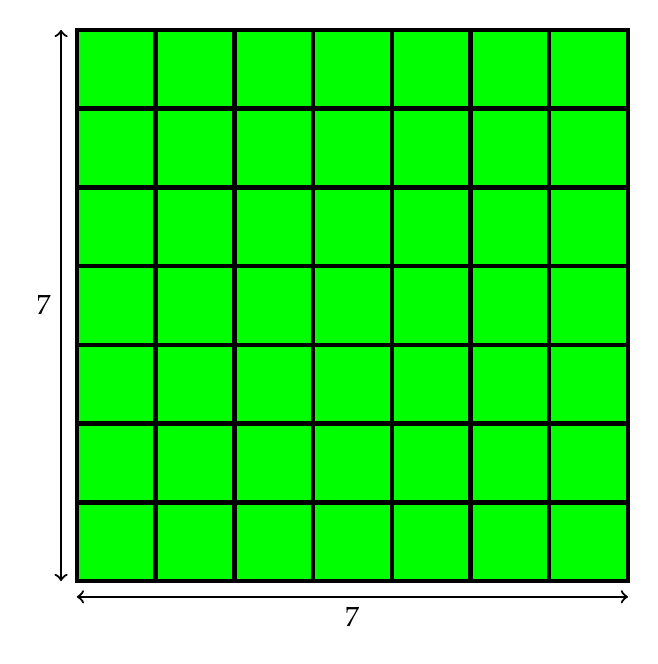
\begin{tikzpicture}
				\foreach \idy [count=\j] in {4,2,...,0}
				{
					\foreach \idx [count=\i] in {0,2,...,4}
					{
						\pgfmathparse{int(\j*3-3+\i)}
						\only<\pgfmathresult>{
							\draw[fill=green, draw=black, ultra thick] (\idx,\idy) rectangle (\idx+3,\idy+3);
						}
						\typeout{\pgfmathresult}
					}
				}
				\foreach \y in {1,...,7} {
					\foreach \x in {1,...,7} {
						\draw [draw=black, ultra thick] (\x-1,\y-1) rectangle (\x,\y);
					}
				}
				\draw[yshift=-0.2cm, thick, <->] (0,0) -- (7,0) node[midway,below] {7};
				\draw[xshift=-0.2cm, thick, <->] (0,0) -- (0,7) node[midway,left] {7};
			\end{tikzpicture}
		}
	\end{center}
\end{frame}

%%%%%%%%%%%%%%%%%%%%%%%%%%%%%%%%%%%%%%%%%%%%%%%%%%%%%%
%%%%%%%%%%%%%%%%%%%%%%%%%%%%%%%%%%%%%%%%%%%%%%%%%%%%%%
\begin{frame}{Convolution}
	\begin{itemize}
		\item 7x7 input.
		\item 3x3 filter.
		\item Stride of 2.
		\item \textbf{3x3 output}.
	\end{itemize}
\end{frame}

%%%%%%%%%%%%%%%%%%%%%%%%%%%%%%%%%%%%%%%%%%%%%%%%%%%%%%
%%%%%%%%%%%%%%%%%%%%%%%%%%%%%%%%%%%%%%%%%%%%%%%%%%%%%%
\subsection{Dimensions}
\begin{frame}{Convolution}
	\begin{columns}[T]
		\begin{column}{.48\textwidth}
			\begin{center}
				\resizebox{!}{\columnwidth}{
					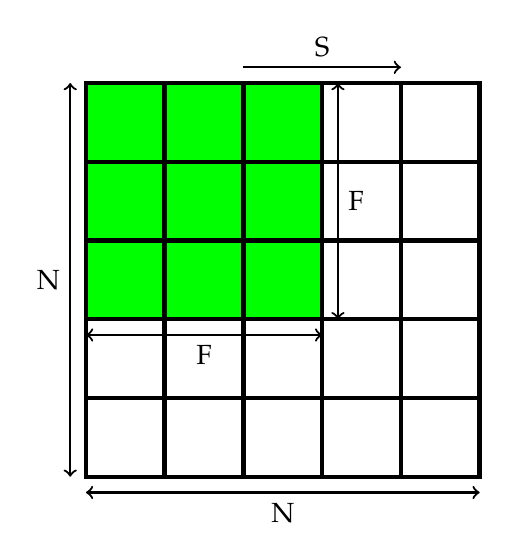
\begin{tikzpicture}
						\draw[fill=green, draw=black, ultra thick] (0,5) rectangle (3,2);
						\foreach \y in {1,...,5} {
							\foreach \x in {1,...,5} {
								\draw [draw=black, ultra thick] (\x-1,\y-1) rectangle (\x,\y);
							}
						}
						\draw[yshift=-0.2cm, thick, <->] (0,0) -- (5,0) node[midway,below] {N};
						\draw[xshift=-0.2cm, thick, <->] (0,0) -- (0,5) node[midway,left] {N};
						\draw[yshift=-0.2cm, thick, <->] (0,2) -- (3,2) node[midway,below] {F};
						\draw[xshift=0.2cm, thick, <->] (3,2) -- (3,5) node[midway,right] {F};
						\draw[yshift=0.2cm, thick, ->] (2,5) -- (4,5) node[midway,above] {S};
					\end{tikzpicture}
				}
			\end{center}
		\end{column}
		\begin{column}{.48\textwidth}
			\begin{itemize}
				\item Output size:
				      \begin{gather*}
				      	\dfrac{N-F}{S}+1
				      \end{gather*}
				      \item<2> First example:
				      \begin{gather*}
				      	\dfrac{7-3}{2}+1 = 3
				      \end{gather*}
				      \item<3> Second example:
				      \begin{gather*}
				      	\dfrac{7-3}{1}+1 = 5
				      \end{gather*}
			\end{itemize}

		\end{column}
	\end{columns}
\end{frame}

%%%%%%%%%%%%%%%%%%%%%%%%%%%%%%%%%%%%%%%%%%%%%%%%%%%%%%
%%%%%%%%%%%%%%%%%%%%%%%%%%%%%%%%%%%%%%%%%%%%%%%%%%%%%%
\begin{frame}{Convolution}
	\begin{itemize}
		\item Sobel filter kept the original image size!
		      \item<2-> Images are usually 0-padded beforehand
	\end{itemize}
	\uncover<2->{
		\begin{columns}[T]
			\begin{column}{.48\textwidth}
				\begin{center}
					\resizebox{!}{\columnwidth}{
						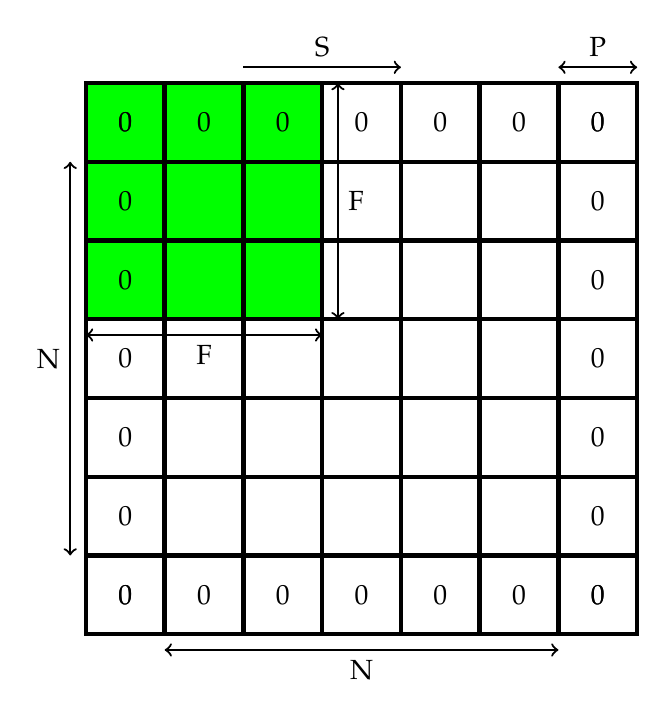
\begin{tikzpicture}
							\draw[fill=green, draw=black, ultra thick] (0,6) rectangle (3,3);
							\foreach \y in {1,...,5} {
								\foreach \x in {2,...,6} {
									\draw [draw=black, ultra thick] (\x-1,\y-1) rectangle (\x,\y);
								}
							}
							\foreach \x in {0,6} {
								\foreach \y in {0,...,6} {
									\draw [draw=black, ultra thick] (\x,\y-1) rectangle (\x+1,\y) node[midway] {0};
								}
							}
							\foreach \y in {0,6} {
								\foreach \x in {0,...,6} {
									\draw [draw=black, ultra thick] (\x,\y-1) rectangle (\x+1,\y) node[midway] {0};
								}
							}
							\draw[yshift=-0.2cm, thick, <->] (1,-1) -- (6,-1) node[midway,below] {N};
							\draw[xshift=-0.2cm, thick, <->] (0,0) -- (0,5) node[midway,left] {N};
							\draw[yshift=-0.2cm, thick, <->] (0,3) -- (3,3) node[midway,below] {F};
							\draw[xshift=0.2cm, thick, <->] (3,3) -- (3,6) node[midway,right] {F};
							\draw[yshift=0.2cm, thick, ->] (2,6) -- (4,6) node[midway,above] {S};
							\draw[yshift=0.2cm, thick, <->] (6,6) -- (7,6) node[midway,above] {P};
						\end{tikzpicture}
					}
				\end{center}
			\end{column}
			\begin{column}{.48\textwidth}
				\begin{itemize}
					\item Output size:
					      \begin{gather*}
					      	\dfrac{N-F+2P}{S}+1
					      \end{gather*}
					      \item<3-> First example with padding:
					      \begin{gather*}
					      	\dfrac{7-3+2}{1}+1 = 7
					      \end{gather*}
					      \begin{itemize}
					      	\item<4-> Original dimension is maintained!
					      \end{itemize}
				\end{itemize}
			\end{column}
		\end{columns}}
\end{frame}

%%%%%%%%%%%%%%%%%%%%%%%%%%%%%%%%%%%%%%%%%%%%%%%%%%%%%%
%%%%%%%%%%%%%%%%%%%%%%%%%%%%%%%%%%%%%%%%%%%%%%%%%%%%%%
\section{\scshape Pooling}
\begin{frame}{Pooling}
	\begin{itemize}
		\item Pooling is a form of non-linear downsampling.
		\item Useful in reducing the size of representations and parameters, therefore reducing the computation required and the chances of overfit.
		\item Also provides a form of translation invariance.
	\end{itemize}
\end{frame}

%%%%%%%%%%%%%%%%%%%%%%%%%%%%%%%%%%%%%%%%%%%%%%%%%%%%%%
%%%%%%%%%%%%%%%%%%%%%%%%%%%%%%%%%%%%%%%%%%%%%%%%%%%%%%
\subsection{Max Pooling}
\begin{frame}{Max Pooling}
	\begin{center}
		\resizebox{\columnwidth}{!}{
			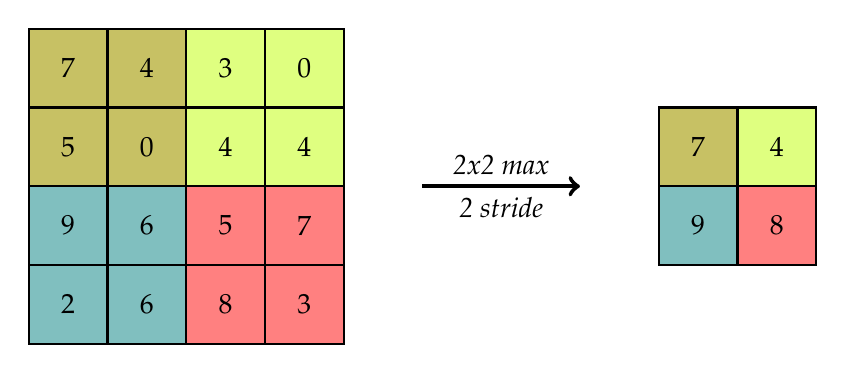
\begin{tikzpicture}
				\draw [draw=black, fill=teal!50, thick] (0,0) rectangle (1,1) node[midway] {2};
				\draw [draw=black, fill=teal!50, thick] (1,0) rectangle (2,1) node[midway] {6};
				\draw [draw=black, fill=teal!50, thick] (0,1) rectangle (1,2) node[midway] {9};
				\draw [draw=black, fill=teal!50, thick] (1,1) rectangle (2,2) node[midway] {6};

				\draw [draw=black, fill=red!50, thick] (2,0) rectangle (3,1) node[midway] {8};
				\draw [draw=black, fill=red!50, thick] (3,0) rectangle (4,1) node[midway] {3};
				\draw [draw=black, fill=red!50, thick] (2,1) rectangle (3,2) node[midway] {5};
				\draw [draw=black, fill=red!50, thick] (3,1) rectangle (4,2) node[midway] {7};

				\draw [draw=black, fill=olive!50, thick] (0,2) rectangle (1,3) node[midway] {5};
				\draw [draw=black, fill=olive!50, thick] (1,2) rectangle (2,3) node[midway] {0};
				\draw [draw=black, fill=olive!50, thick] (0,3) rectangle (1,4) node[midway] {7};
				\draw [draw=black, fill=olive!50, thick] (1,3) rectangle (2,4) node[midway] {4};

				\draw [draw=black, fill=lime!50, thick] (2,2) rectangle (3,3) node[midway] {4};
				\draw [draw=black, fill=lime!50, thick] (3,2) rectangle (4,3) node[midway] {4};
				\draw [draw=black, fill=lime!50, thick] (2,3) rectangle (3,4) node[midway] {3};
				\draw [draw=black, fill=lime!50, thick] (3,3) rectangle (4,4) node[midway] {0};

				\draw[ultra thick, ->] (5,2) -- (7,2) node[midway,above] {\textit{2x2 max}} node[midway,below] {\textit{2 stride}};

				\draw [draw=black, fill=teal!50, thick] (8,1) rectangle (9,2) node[midway] {9};
				\draw [draw=black, fill=red!50, thick] (9,1) rectangle (10,2) node[midway] {8};
				\draw [draw=black, fill=olive!50, thick] (8,2) rectangle (9,3) node[midway] {7};
				\draw [draw=black, fill=lime!50, thick] (9,2) rectangle (10,3) node[midway] {4};
			\end{tikzpicture}
		}
	\end{center}
\end{frame}

%%%%%%%%%%%%%%%%%%%%%%%%%%%%%%%%%%%%%%%%%%%%%%%%%%%%%%
%%%%%%%%%%%%%%%%%%%%%%%%%%%%%%%%%%%%%%%%%%%%%%%%%%%%%%
\subsection{Average Pooling}
\begin{frame}{Average Pooling}
	\begin{center}
		\resizebox{\columnwidth}{!}{
			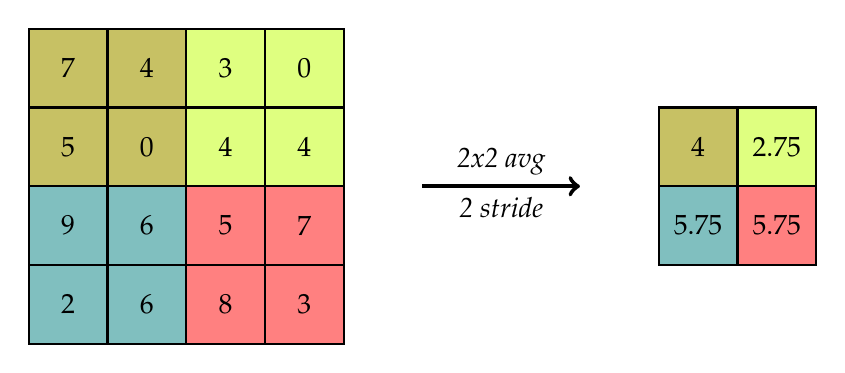
\begin{tikzpicture}
				\draw [draw=black, fill=teal!50, thick] (0,0) rectangle (1,1) node[midway] {2};
				\draw [draw=black, fill=teal!50, thick] (1,0) rectangle (2,1) node[midway] {6};
				\draw [draw=black, fill=teal!50, thick] (0,1) rectangle (1,2) node[midway] {9};
				\draw [draw=black, fill=teal!50, thick] (1,1) rectangle (2,2) node[midway] {6};

				\draw [draw=black, fill=red!50, thick] (2,0) rectangle (3,1) node[midway] {8};
				\draw [draw=black, fill=red!50, thick] (3,0) rectangle (4,1) node[midway] {3};
				\draw [draw=black, fill=red!50, thick] (2,1) rectangle (3,2) node[midway] {5};
				\draw [draw=black, fill=red!50, thick] (3,1) rectangle (4,2) node[midway] {7};

				\draw [draw=black, fill=olive!50, thick] (0,2) rectangle (1,3) node[midway] {5};
				\draw [draw=black, fill=olive!50, thick] (1,2) rectangle (2,3) node[midway] {0};
				\draw [draw=black, fill=olive!50, thick] (0,3) rectangle (1,4) node[midway] {7};
				\draw [draw=black, fill=olive!50, thick] (1,3) rectangle (2,4) node[midway] {4};

				\draw [draw=black, fill=lime!50, thick] (2,2) rectangle (3,3) node[midway] {4};
				\draw [draw=black, fill=lime!50, thick] (3,2) rectangle (4,3) node[midway] {4};
				\draw [draw=black, fill=lime!50, thick] (2,3) rectangle (3,4) node[midway] {3};
				\draw [draw=black, fill=lime!50, thick] (3,3) rectangle (4,4) node[midway] {0};

				\draw[ultra thick, ->] (5,2) -- (7,2) node[midway,above] {\textit{2x2 avg}} node[midway,below] {\textit{2 stride}};

				\draw [draw=black, fill=teal!50, thick] (8,1) rectangle (9,2) node[midway] {5.75};
				\draw [draw=black, fill=red!50, thick] (9,1) rectangle (10,2) node[midway] {5.75};
				\draw [draw=black, fill=olive!50, thick] (8,2) rectangle (9,3) node[midway] {4};
				\draw [draw=black, fill=lime!50, thick] (9,2) rectangle (10,3) node[midway] {2.75};
			\end{tikzpicture}
		}
	\end{center}
\end{frame}

%%%%%%%%%%%%%%%%%%%%%%%%%%%%%%%%%%%%%%%%%%%%%%%%%%%%%%
%%%%%%%%%%%%%%%%%%%%%%%%%%%%%%%%%%%%%%%%%%%%%%%%%%%%%%
\begin{frame}{Pooling}
	\begin{itemize}
		\item In practice max pooling has been shown to work better.
		      \begin{itemize}
		      	\item Pixels are highly co-dependent, therefore the same feature is seldom found twice in close promixity.
		      	\item Since all we are concerned about is whether or not a feature is present, taking the average would just reduce the activation magnitude.
		      	      \begin{itemize}
		      	      	\item Imagine a population of 5 and we want to know if zika is present. If at least one person has it, we say yes. You wouldn't count the occurrences and divide by 5.
		      	      \end{itemize}
		      \end{itemize}
	\end{itemize}
\end{frame}

%%%%%%%%%%%%%%%%%%%%%%%%%%%%%%%%%%%%%%%%%%%%%%%%%%%%%%
%%%%%%%%%%%%%%%%%%%%%%%%%%%%%%%%%%%%%%%%%%%%%%%%%%%%%%
\section{\scshape Convolutional Neural Networks}
\begin{frame}{Convolutional Neural Networks}
	\begin{itemize}
		\item Putting it all together, we have convolutional neural networks.
	\end{itemize}
	\begin{center}
		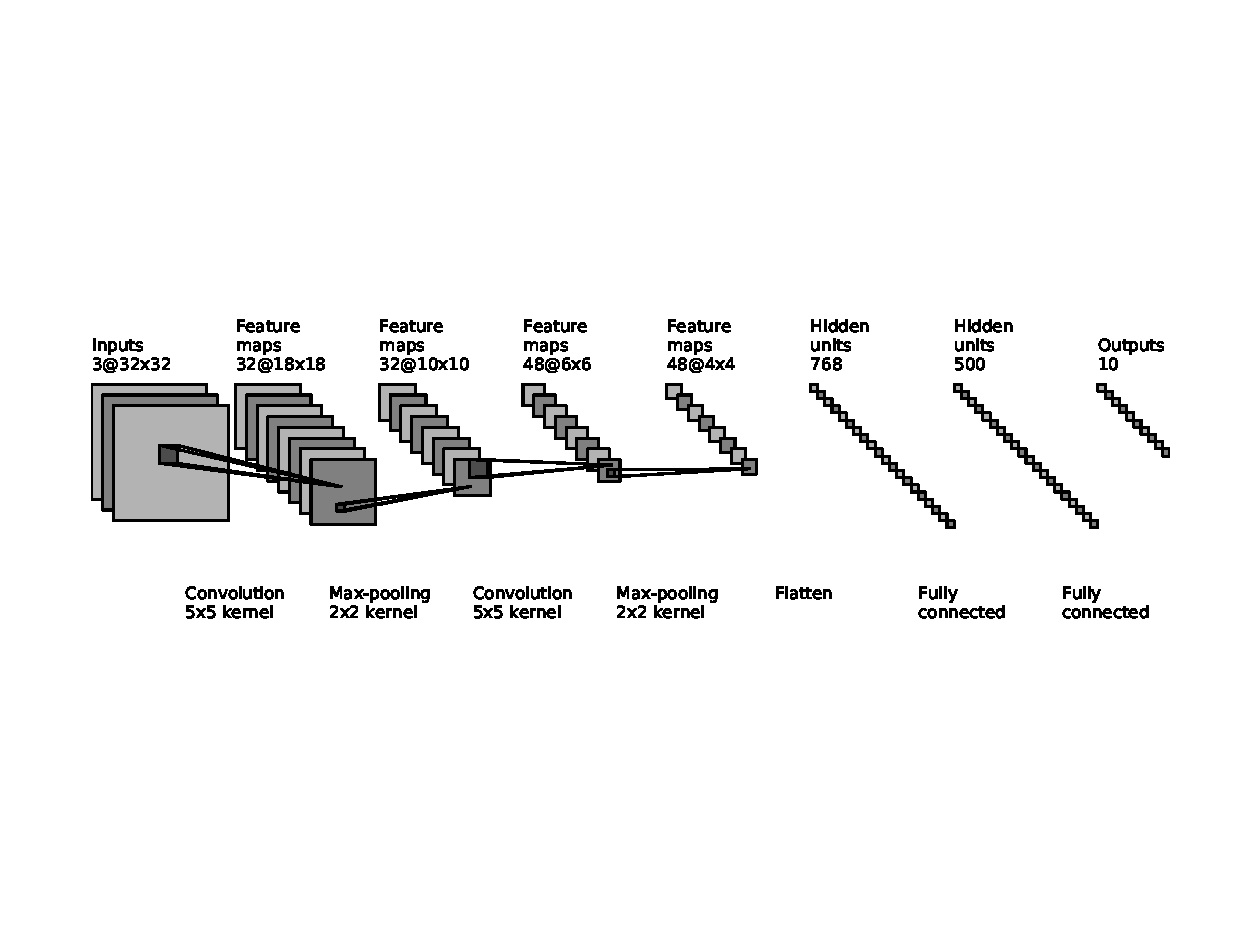
\includegraphics[width=\columnwidth,trim={1cm 4cm 0 4cm},clip]{convnet.eps}
	\end{center}
	\begin{itemize}
		\item New types of layers: Convolution and Pooling.
	\end{itemize}
\end{frame}

%%%%%%%%%%%%%%%%%%%%%%%%%%%%%%%%%%%%%%%%%%%%%%%%%%%%%%
%%%%%%%%%%%%%%%%%%%%%%%%%%%%%%%%%%%%%%%%%%%%%%%%%%%%%%
\begin{frame}{Convolutional Neural Networks}
	\begin{itemize}
		\item Convolution layers compute feature maps from the image response to multiple filters.
		      \begin{itemize}
		      	\item These filters can be learned automatically with gradient descent!
		      \end{itemize}
		\item Pooling layers subsample these feature maps, usually taking the max.
		      \begin{itemize}
		      	\item Provides translation and rotation \textit{in}variance.
		      \end{itemize}
	\end{itemize}
\end{frame}

%%%%%%%%%%%%%%%%%%%%%%%%%%%%%%%%%%%%%%%%%%%%%%%%%%%%%%
%%%%%%%%%%%%%%%%%%%%%%%%%%%%%%%%%%%%%%%%%%%%%%%%%%%%%%
\begin{frame}{Convolutional Neural Networks}
	\begin{itemize}
		\item It is possible to compute the same outputs of a convolutional layer using a fully connected layer.
		      \begin{itemize}
		      	\item Much bigger network and therefore harder to train.
		      	\item Also more susceptible to overfitting.
		      \end{itemize}
		\item Convolutional Neural Networks have fewer parameters due to \textbf{weight sharing}.
	\end{itemize}
\end{frame}

%%%%%%%%%%%%%%%%%%%%%%%%%%%%%%%%%%%%%%%%%%%%%%%%%%%%%%
%%%%%%%%%%%%%%%%%%%%%%%%%%%%%%%%%%%%%%%%%%%%%%%%%%%%%%
\subsection{Backpropagation}
\begin{frame}{Tiny CNN}
	\begin{center}
		\begin{tikzpicture}[shorten >=1pt,->,draw=black!50, node distance=\layersep]
			\tikzstyle{every pin edge}=[<-,shorten <=1pt]
			\tikzstyle{neuron}=[circle,draw=black!25,minimum size=17pt,inner sep=0pt]
			\tikzstyle{input neuron}=[neuron, fill=yellow!50];
			\tikzstyle{conv neuron}=[neuron, fill=green!75];
			\tikzstyle{max neuron}=[neuron, fill=red!75];
			\tikzstyle{output neuron}=[neuron, fill=orange!50];
			\tikzstyle{annot} = [text width=5em, text centered]

			\foreach \name / \x in {1,...,4}
			\node[input neuron, pin=left:$x^{(i)}_\x$] (I-\name) at (0,-\x) {};

			\foreach \name / \x in {1,...,3}
			\path[yshift=-0.5cm]
			node[conv neuron] (H-\name) at (\layersep,-\x) {};

			\foreach \name [count=\i] in {1,...,3}
			{
				\draw[->] (I-\i) -- (H-\name) node[midway,xshift=0.1cm] {$\boldsymbol{W_1}$};
				\pgfmathparse{int(1+\i)}
				\draw[->] (I-\pgfmathresult) -- (H-\name) node[midway,xshift=-0.1cm] {$\boldsymbol{W_2}$};
			}

			\foreach \name / \x in {1,...,2}
			\path[yshift=-1cm]
			node[max neuron] (M-\name) at (2*\layersep,-\x) {};

			\foreach \name [count=\i] in {1,...,2}
			{
				\draw[->] (H-\i) -- (M-\name);
				\pgfmathparse{int(1+\i)}
				\draw[->] (H-\pgfmathresult) -- (M-\name) node[midway,yshift=0.25cm] {\textit{max}};
			}
			\node[annot,above of=I-1,node distance=1cm] (IL) {Input};
			\node[annot,right of=IL] (CL) {Convolution Layer};
			\node[annot,right of=CL] (ML) {Max-Pool Layer};
		\end{tikzpicture}
	\end{center}
\end{frame}

%%%%%%%%%%%%%%%%%%%%%%%%%%%%%%%%%%%%%%%%%%%%%%%%%%%%%%
%%%%%%%%%%%%%%%%%%%%%%%%%%%%%%%%%%%%%%%%%%%%%%%%%%%%%%
\begin{frame}{Backpropagation in Tiny CNN}
	{\center Convolution Layers\par}
	\begin{columns}[T]
		\begin{column}{0.48\textwidth}
			\begin{center}
				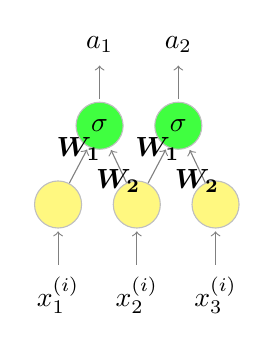
\begin{tikzpicture}[shorten >=1pt,->,draw=black!50, node distance=\layersep]
					\tikzstyle{every pin edge}=[<-,shorten <=1pt]
					\tikzstyle{neuron}=[circle,draw=black!25,minimum size=17pt,inner sep=0pt]
					\tikzstyle{input neuron}=[neuron, fill=yellow!50];
					\tikzstyle{conv neuron}=[neuron, fill=green!75];
					\tikzstyle{max neuron}=[neuron, fill=red!75];
					\tikzstyle{output neuron}=[neuron, fill=orange!50];
					\tikzstyle{annot} = [text width=5em, text centered]

					\foreach \name / \x in {1,...,3}
					\node[input neuron, pin=below:$x^{(i)}_\x$] (I-\name) at (\x,0) {};

					\foreach \name / \x in {1,2}
					\path[xshift=15pt]
					node[conv neuron, pin={[pin edge={->}]above:$a_\x$}] (H-\x) at (\x,\layersep) {$\sigma$};

					\draw[->] (I-1) -- (H-1) node[midway, yshift=0.2cm] {$\boldsymbol{W_1}$};
					\draw[->] (I-2) -- (H-1) node[midway, yshift=-0.2cm] {$\boldsymbol{W_2}$};
					\draw[->] (I-2) -- (H-2) node[midway, yshift=0.2cm] {$\boldsymbol{W_1}$};
					\draw[->] (I-3) -- (H-2) node[midway, yshift=-0.2cm] {$\boldsymbol{W_2}$};
				\end{tikzpicture}
			\end{center}
		\end{column}
		\begin{column}{0.48\textwidth}
			\begin{alignat}{2}
				\notag a_1                               & = \sigma(W_1.x_1 + W_2.x_2)                     \\
				\notag \frac{\partial a_1}{\partial w_1} & = x_1\sigma'(W_1.x_1 + W_2.x_2)
				\\
				\notag \frac{\partial a_2}{\partial w_1} & = x_2\sigma'(W_1.x_2 + W_2.x_3)
				\\
				\notag \frac{\partial a}{\partial w_1} & = \frac{\partial a_2}{\partial w_1} + \frac{\partial a_1}{\partial w_1}           
			\end{alignat}
		\end{column}
	\end{columns}
\end{frame}


%%%%%%%%%%%%%%%%%%%%%%%%%%%%%%%%%%%%%%%%%%%%%%%%%%%%%%
%%%%%%%%%%%%%%%%%%%%%%%%%%%%%%%%%%%%%%%%%%%%%%%%%%%%%%
\begin{frame}{Backpropagation in Tiny CNN}
	{\center Max-Pool Layers\par}
	\begin{columns}[T]
		\begin{column}{0.48\textwidth}
			\begin{center}
				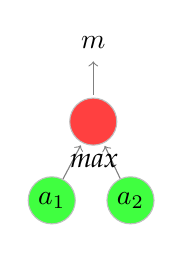
\begin{tikzpicture}[shorten >=1pt,->,draw=black!50, node distance=\layersep]
					\tikzstyle{every pin edge}=[<-,shorten <=1pt]
					\tikzstyle{neuron}=[circle,draw=black!25,minimum size=17pt,inner sep=0pt]
					\tikzstyle{input neuron}=[neuron, fill=yellow!50];
					\tikzstyle{conv neuron}=[neuron, fill=green!75];
					\tikzstyle{max neuron}=[neuron, fill=red!75];
					\tikzstyle{output neuron}=[neuron, fill=orange!50];
					\tikzstyle{annot} = [text width=5em, text centered]

					\foreach \name / \x in {1,2}
					\node[conv neuron] (I-\name) at (\x,0) {$a_\name$};

					\path[xshift=15pt]
					node[max neuron, pin={[pin edge={->}]above:$m$}] (H-1) at (1,\layersep) {};

					\draw[->] (I-1) -- (H-1);
					\draw[->] (I-2) -- (H-1) node[midway,left,xshift=0.2cm] {\textit{max}};
				\end{tikzpicture}
			\end{center}
		\end{column}
		\begin{column}{0.48\textwidth}
			\begin{gather*}
				m = max(a_1, a_2)\\
				\frac{\partial m}{\partial a_i} = \begin{dcases}1 &a_i>a_j, \forall i \neq j\\ 0 & otherwise\end{dcases}
			\end{gather*}
			\begin{itemize}
				\item $a$s are real, so we don't need to worry about them being equal.
				\item With this scheme the gradient flows only to the neuron responsible for the value of m.
			\end{itemize}
		\end{column}
	\end{columns}
\end{frame}

%%%%%%%%%%%%%%%%%%%%%%%%%%%%%%%%%%%%%%%%%%%%%%%%%%%%%%
%%%%%%%%%%%%%%%%%%%%%%%%%%%%%%%%%%%%%%%%%%%%%%%%%%%%%%
\subsection{Dataset Augmentation}
\begin{frame}{Dataset Augmentation}
	\begin{itemize}
		\item Convolutional Networks distinguish themselves by how well they handle translation, rotation and scale variances.
		\item We can further encourage this behavior by performing \textbf{data augmentation}. Which consists of purposely adding variations to the dataset.
		      \begin{itemize}
		      	\item Repeat certain inputs in different scales, mirrored, skewed, rotated, etc.
		      \end{itemize}
		\item Since more data (albeit artificial) becomes available, overfitting becomes harder.
	\end{itemize}
\end{frame}

%%%%%%%%%%%%%%%%%%%%%%%%%%%%%%%%%%%%%%%%%%%%%%%%%%%%%%
%%%%%%%%%%%%%%%%%%%%%%%%%%%%%%%%%%%%%%%%%%%%%%%%%%%%%%
\subsection{Bag of Tricks}
\begin{frame}{Bag of Tricks}
	\begin{itemize}
		\item Previously discussed training methods still apply here:
		\item Gradient descent is used to train the network end-to-end.
		\item Dropout or L2/L1 regularization is applied to fully connected layers to prevent overfitting.
		\item Data normalization.
	\end{itemize}
\end{frame}

%%%%%%%%%%%%%%%%%%%%%%%%%%%%%%%%%%%%%%%%%%%%%%%%%%%%%%
%%%%%%%%%%%%%%%%%%%%%%%%%%%%%%%%%%%%%%%%%%%%%%%%%%%%%%
\subsection{Code Example}
\begin{frame}{Code Example}
	\begin{itemize}
		\item Open a terminal and type:
	\end{itemize}
	\begin{center}
		{\smaller \texttt{python -m tensorflow.models.image.mnist.convolutional}}
	\end{center}
\end{frame}

%%%%%%%%%%%%%%%%%%%%%%%%%%%%%%%%%%%%%%%%%%%%%%%%%%%%%%
%%%%%%%%%%%%%%%%%%%%%%%%%%%%%%%%%%%%%%%%%%%%%%%%%%%%%%
\begin{frame}{MNIST}
	\begin{itemize}
		\item Comparative table of our models so far:
	\end{itemize}
	\begin{table}[]
		\centering
		\begin{tabular}{lll}
			\cline{2-3}
			                               & Train  & Test    \\ \hline
			Logistic Regression            & 94.1\% & 92.11\% \\
			Fully Connected Neural Network & 100\%  & 95.6\%  \\
			Convolutional Neural Network   & 100\%  & 99.2\%  \\ \hline
		\end{tabular}
	\end{table}
\end{frame}

%%%%%%%%%%%%%%%%%%%%%%%%%%%%%%%%%%%%%%%%%%%%%%%%%%%%%%
%%%%%%%%%%%%%%%%%%%%%%%%%%%%%%%%%%%%%%%%%%%%%%%%%%%%%%
\begin{frame}{Fun}
	\begin{center}
		\textcolor{blue!75}{\underline{ \href{http://nightmare.mit.edu/}{MIT's Nightmare Machine}}}
	\end{center}
\end{frame}

\end{document}
